\documentclass[11pt]{article}
\usepackage[utf8]{inputenc}
\usepackage[english]{babel}
\usepackage[
backend=biber,
style=alphabetic,
sorting=ynt
]{biblatex}
\addbibresource{references.bib}
\usepackage{amsmath}  % Basic math symbols and environments
\usepackage{amssymb}  % Extended symbol collection
\usepackage{mathtools} % Fixes and additions to amsmath
\usepackage{algorithm}
\usepackage{algpseudocode}
\usepackage{graphicx}
\usepackage{float}
\usepackage{csvsimple}
\usepackage[colorlinks=true]{hyperref}
\usepackage{indentfirst}
\usepackage{listings}
\newlength{\Lnote}
\newcommand{\note}[1]
{\addtolength{\leftmargini}{4em}
	\settowidth{\Lnote}{\textbf{Note:~}}
	\begin{quote}
		\rule{\dimexpr\textwidth-2\leftmargini}{1pt}\\
		\mbox{}\hspace{-\Lnote}\textbf{Note:~}%
		#1\\[-0.5ex] 
		\rule{\dimexpr\textwidth-2\leftmargini}{1pt}
	\end{quote}
	\addtolength{\leftmargini}{-4em}}
\begin{document}
\title{AIML427 - Big Data Assignment \#2}
author: Jason Pollock
email: jason@pollock.ca, pollocjaso@myvuw.ac.nz

\section{Manifold Learning}

\subsection{Question 1}
I picked \href{https://archive-beta.ics.uci.edu/dataset/579/myocardial+infarction+complications}{Myocardial infarction complications}. It has 111 features, and 1,700 instances. The purpose of the dataset is to predict complications that a patient will have at admission or the first 24, 48, or 72 hours after admission.

This matches the problem's requirements.

I spent hours searching through NZ Government public datasets, NIWA, NOAA and other official sources of data. None supported searching by "number of features". Eventually I found the University of California Irvine website. 

I have no personal interest in this dataset.

I implemented this using KNIME. A screenshot of the workflow is in the appendix. The workflow is in "AIML\_427\_Assignment\_2\_Manifold\_Learning\_Classic\_Manifold.knwf".

\subsection{Question 2 - PCA}

\begin{figure}[H]
	\centering
	\begin{minipage}{.6\textwidth}
		\centering
		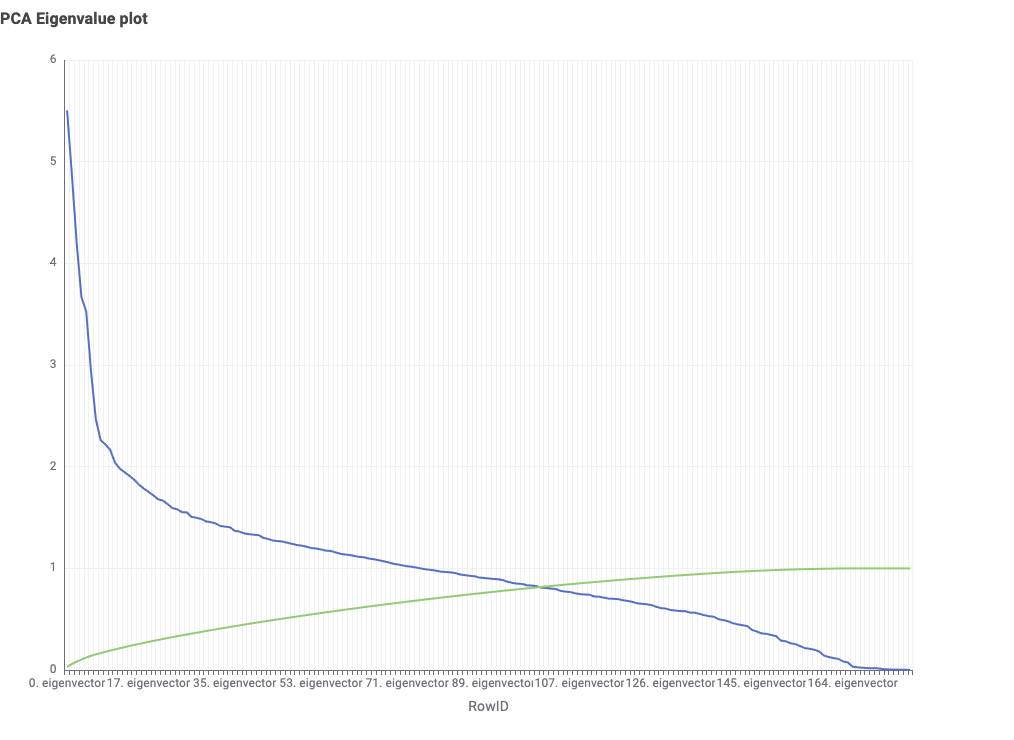
\includegraphics[width=.5\textwidth]{pca_eigenvalue}
		\caption{PCA Eigenvalue Plot}
		\label{fig:1.1}
	\end{minipage}%
	\begin{minipage}{.6\textwidth}
		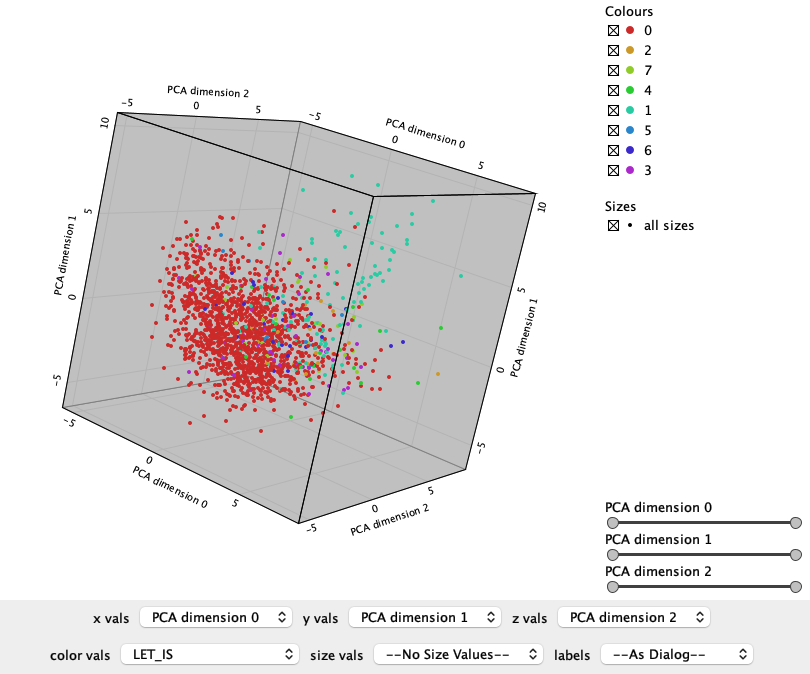
\includegraphics[width=.5\textwidth]{pca_let_is}
		\caption{Top-3 Eigenvalues}
		\label{fig:1.2}
	\end{minipage}
\end{figure}

The top-3 eigenvalues explain only 10\% of the variance in the dataset. 20 vectors are required to explain 30\% of the variance. I found this by summing the eigenvalues and then normalising each eigenvalue by the sum. This creates a column that sums to 1, allowing me to pick the point where the eigenvalue crosses various boundaries. PC1 explains 5/177 = 3\% of the variance.

\subsection{Question 3 - Classic - MDS}

\begin{figure}[H]
	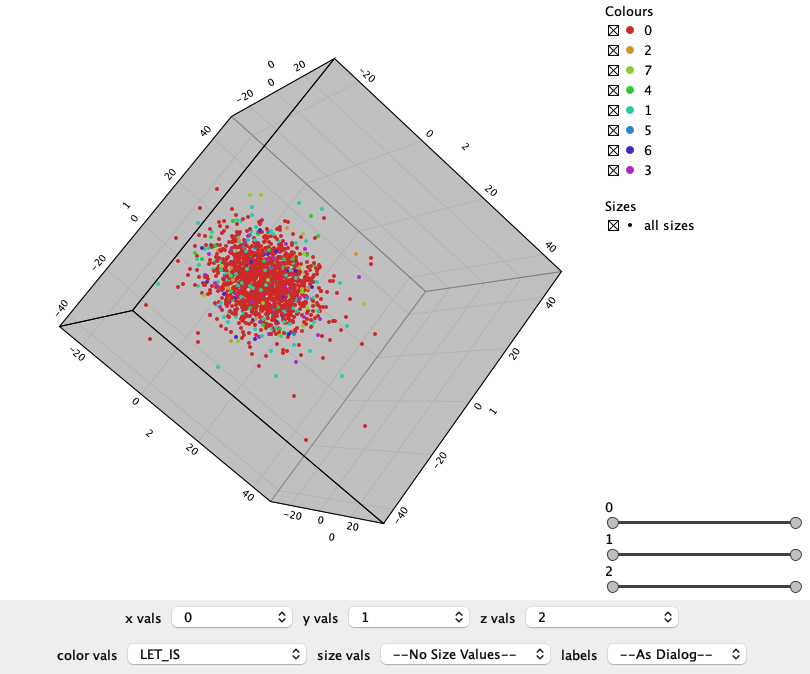
\includegraphics[width=0.4\textwidth]{mds_scatterplot}
	\caption{MDS Manifold to 3 Dimensions}
	\label{fig:1.3}
\end{figure}

The incoming total variance is 176.89, and the outgoing total variance is 163.9. The transformation explains much more of the variance in the incoming dataset \(163.9/176.9 = 92.6\%\).

PCA conversion appears to separate LET\_IS=1 from the other values. The resulting graph does not reveal any separable components. That PCA is able to separate out the one set of values indicates that they are strongly controlled by the values in the first 3 components. It should be possible to take the eigenvectors and extract the largest/smallest coefficients as potential features to attack.

While MDS reduced the dimensions, there is no apparent structure to the results, giving no further clues.

\subsection{Question 4 - Modern - t-SNE}

\begin{figure}[H]
	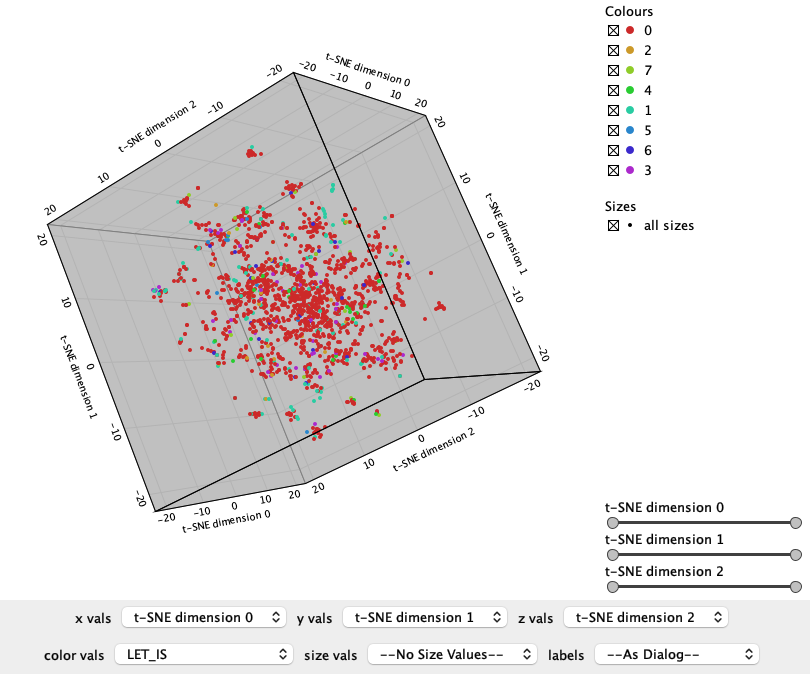
\includegraphics[width=0.4\textwidth]{t-sne}
	\caption{t-SNE to 3 dimensions}
	\label{fig:1.4}
\end{figure}

I tried to use UMap in KNime, but it required setting up a new Python Conda environment, and KNime failed to start the interpreter. I went back to the built-in python environment instead.

t-SNE appears to have produced some clusters. However, the clusters are all in "patient is alive". The interesting clusters, where the patient is dead, show no clustering.

Which is to be expected. If the values were easily clusterable by these algorithms, there would be a sharp decrease in mortality. I believe the algorithm is finding clusters that represent missing data in the raw dataset.

\subsection{Question 4 - Modern - t-SNE hyperparameter tuning}

Plots of each attempt are in the Appendix. I tried the following hyperparameters:

\begin{table}[H]
	\centering
\begin{tabular}{ | c | c | c | }
	\hline
	\textbf{Iterations} & \textbf{Perplexity} & \textbf{theta} \\
	\hline
	100 & 30 & 0.5  \\
	\hline	
	1,000 & 30 & 0.5  \\
	\hline
	10,000 & 30 & 0.5 \\
	\hline
	50,000 & 30 & 0.5 \\
	\hline
	100,000 & 30 & 0.5 \\
	\hline
	1,000 & 2 & 0.5	\\	
	\hline
	1,000 & 5 & 0.5 \\
	\hline
	1,000 & 100 & 0.5 \\
	\hline
	10,000 & 30 & 0.01 \\
	\hline
	10,000 & 2 & 0.01 \\			
	\hline
\end{tabular}
\caption{1.5 t-SNE Hyperparameters.}
\end{table}

I tested the hyperparameter's effects by modifying a KNime workflow to run t-SNE with those values and generate an image.

I initially chose "iterations" for the hyperparameter to tune. None of the hyperparameter values exposed any substantial structure in the dataset. They did make small clumps visible, but nothing general. The iteration count controls the number of times the points are moved down the gradient minimizing the probability distribution difference.

I also varied perplexity - representing the number of neighbours to measure. While all of these varied the resulting graphs, none of them presenting anything informative.

Finally, I modified theta - a value used to increase performance in exchante for accuracy. Instead of calculating the force from all points, it will only consider points that are close to the point being considered.

\section{Clustering}

The code for this section is in \(clustering.ipnyb\). It can be executed using \(make\ all\) or \(make\ part2\).

\subsection{Hierarchical Clustering with Eucliden Distances and Complete Linkage}

\begin{figure}[H]
	\centering
	\begin{minipage}{.5\textwidth}
		\centering
		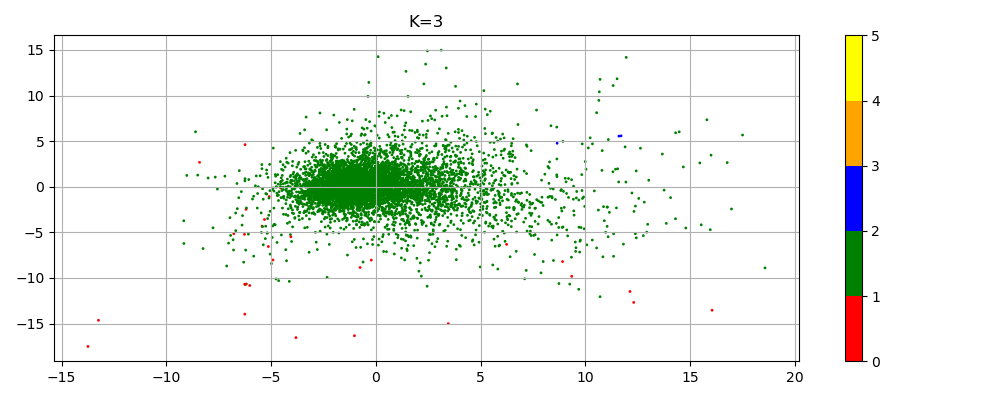
\includegraphics[width=1.0\textwidth]{euclidean_3}
		\caption{Euclidean k=3}
		\label{fig:2.1}
	\end{minipage}%
	\begin{minipage}{.5\textwidth}
		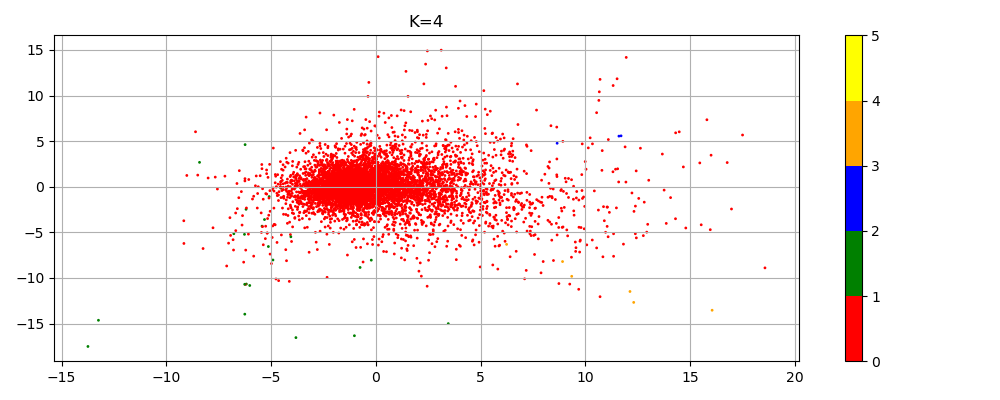
\includegraphics[width=1.0\textwidth]{euclidean_4}
		\caption{Euclidean k=4}
		\label{fig:2.2}
	\end{minipage}
\end{figure}
\begin{figure}[H]
	\centering
	\begin{minipage}{.5\textwidth}
		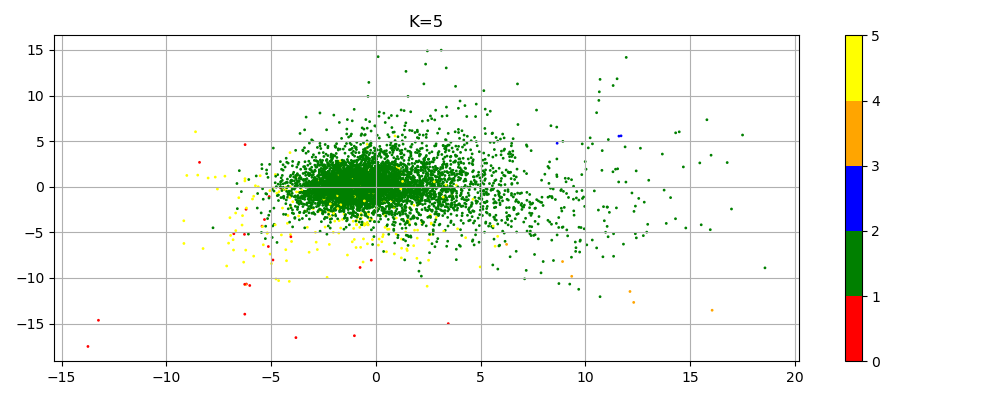
\includegraphics[width=1.0\textwidth]{euclidean_5}
		\caption{Euclidean k=5}
		\label{fig:2.3}
	\end{minipage}%
	\begin{minipage}{.5\textwidth}
		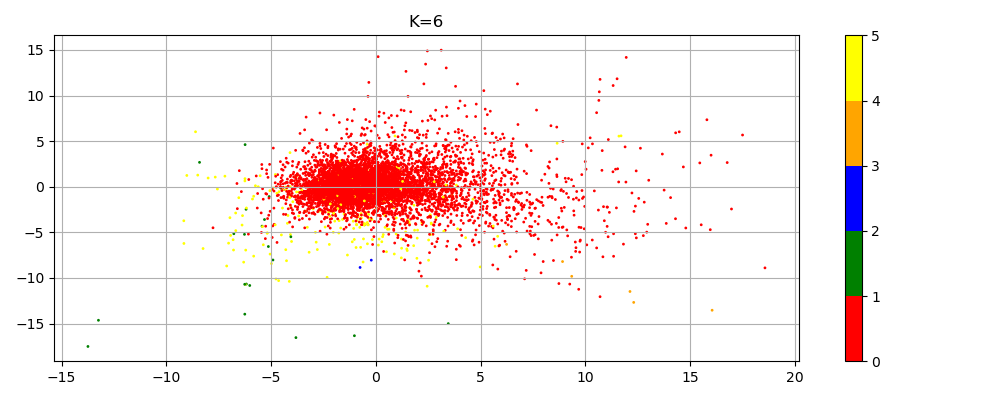
\includegraphics[width=1.0\textwidth]{euclidean_6}
		\caption{Euclidean k=6}
		\label{fig:2.4}
	\end{minipage}
\end{figure}

Euclidean distance doesn't work well with this dataset. That is to be expected since there are lots of dimensions and in high-dimension data most data is close. The plots using the PCA all showed a single primary cluster with a smattering of single point clusters outside of the main cluster.

\subsection{Hierarchical Clustering with Correlation Based Distances and Complete Linkage}

\begin{figure}[H]
	\centering
	\begin{minipage}{.5\textwidth}
		\centering
		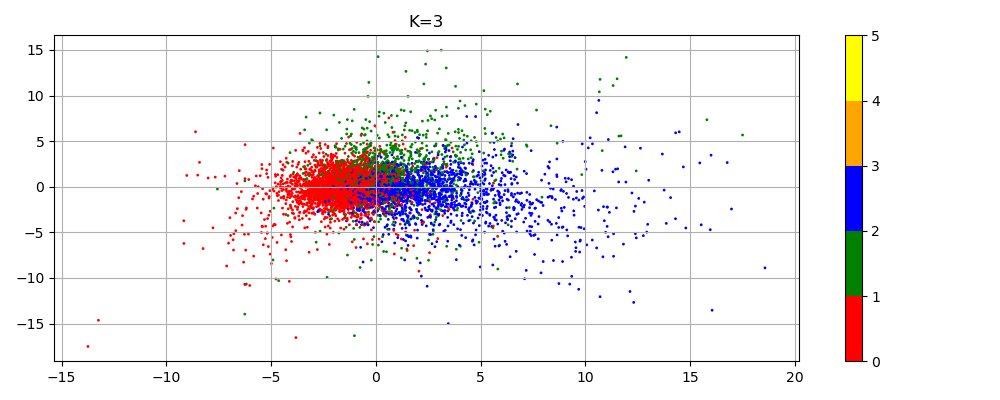
\includegraphics[width=1.0\textwidth]{correlation_3}
		\caption{Correlation k=3}
		\label{fig:2.5}
	\end{minipage}%
	\begin{minipage}{.5\textwidth}
		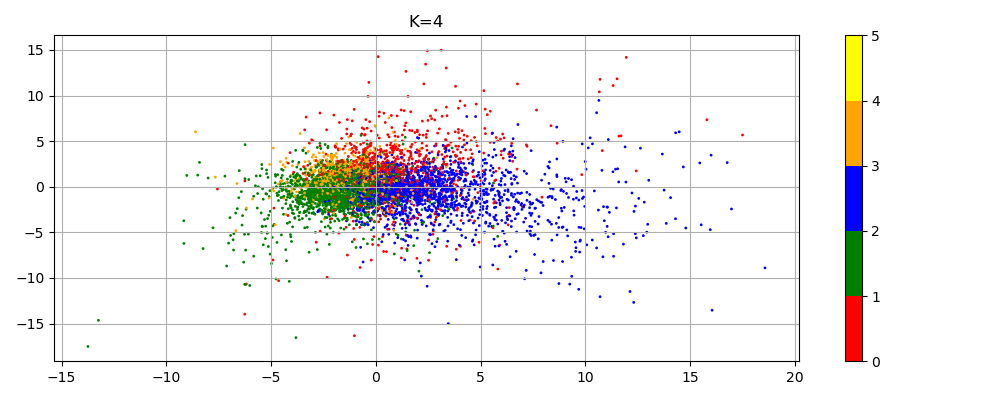
\includegraphics[width=1.0\textwidth]{correlation_4}
		\caption{Correlation k=4}
		\label{fig:2.6}
	\end{minipage}
\end{figure}
\begin{figure}[H]
	\centering
	\begin{minipage}{.5\textwidth}
		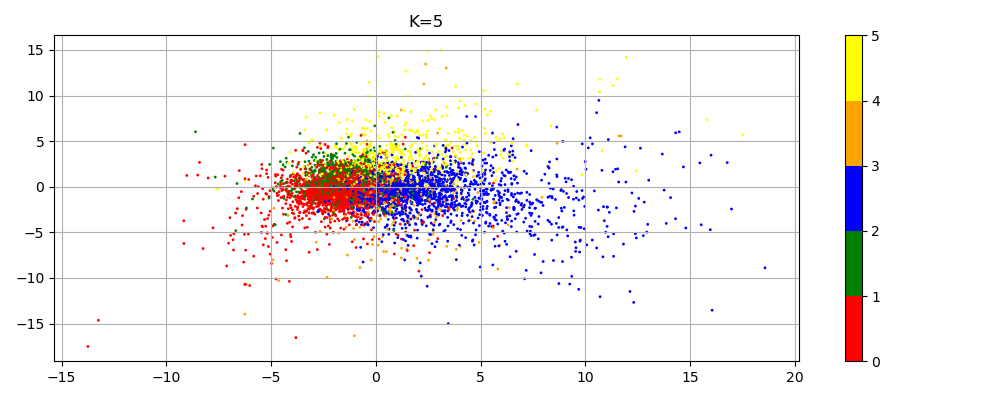
\includegraphics[width=1.0\textwidth]{correlation_5}
		\caption{Correlation k=5}
		\label{fig:2.7}
	\end{minipage}%
	\begin{minipage}{.5\textwidth}
		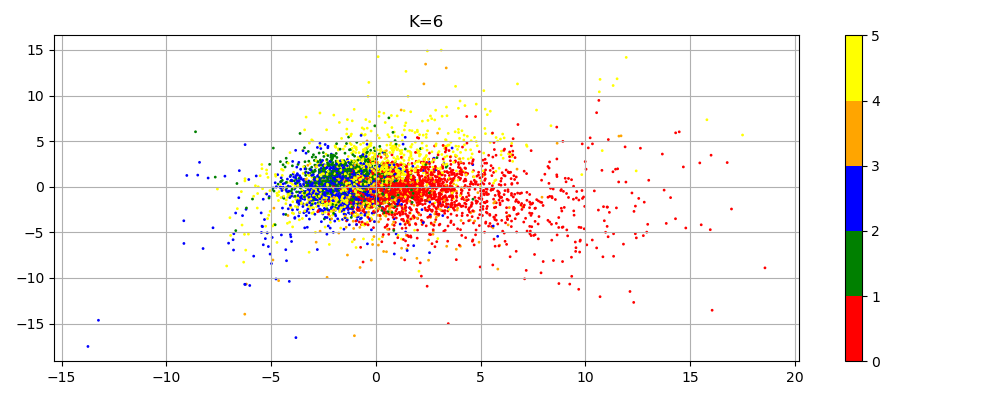
\includegraphics[width=1.0\textwidth]{correlation_6}
		\caption{Correlation k=6}
		\label{fig:2.8}
	\end{minipage}
\end{figure}

Correlation based clusters created clusters. However, they had soft edges and significant overlap when projected into the PCA 2-space. The projection may be working against us, and we should look for metrics to evaluate the cluster in the original N-space, such as silhouette.

\subsection{K-means}

\begin{figure}[H]
	\centering
	\begin{minipage}{.5\textwidth}
		\centering
		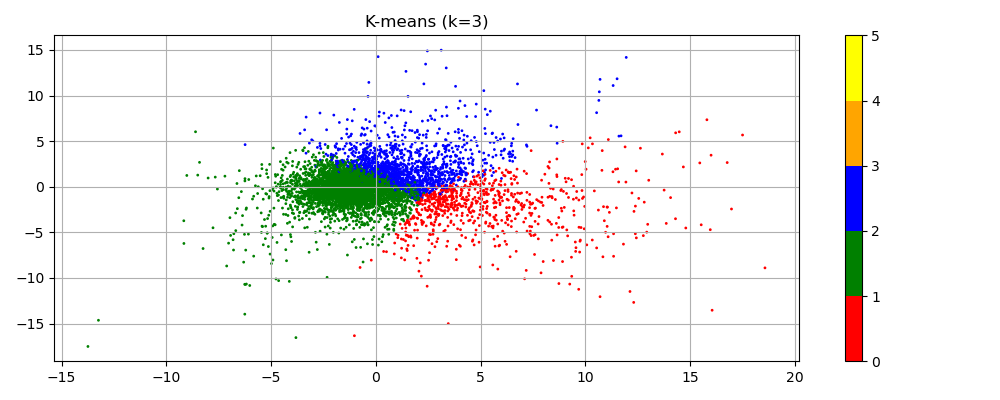
\includegraphics[width=1.0\textwidth]{kmeans_3}
		\caption{K-Means k=3}
		\label{fig:2.9}
	\end{minipage}%
	\begin{minipage}{.5\textwidth}
		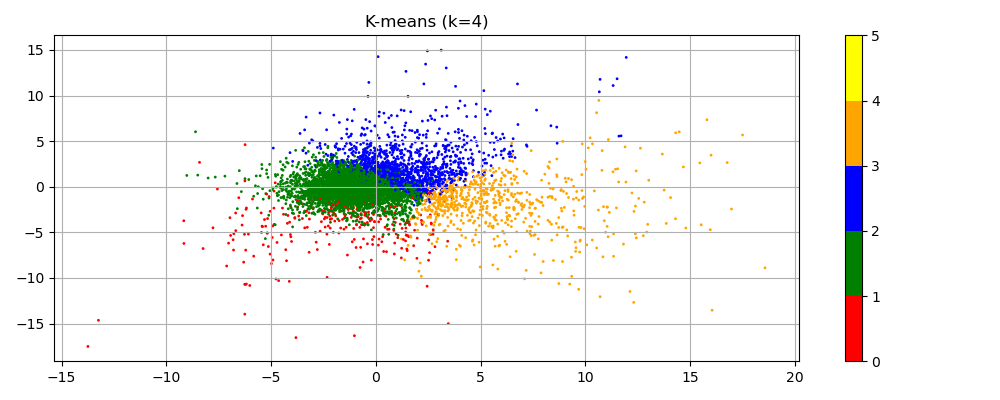
\includegraphics[width=1.0\textwidth]{kmeans_4}
		\caption{K-Means k=4}
		\label{fig:2.10}
	\end{minipage}
\end{figure}
\begin{figure}[H]
	\centering
	\begin{minipage}{.5\textwidth}
		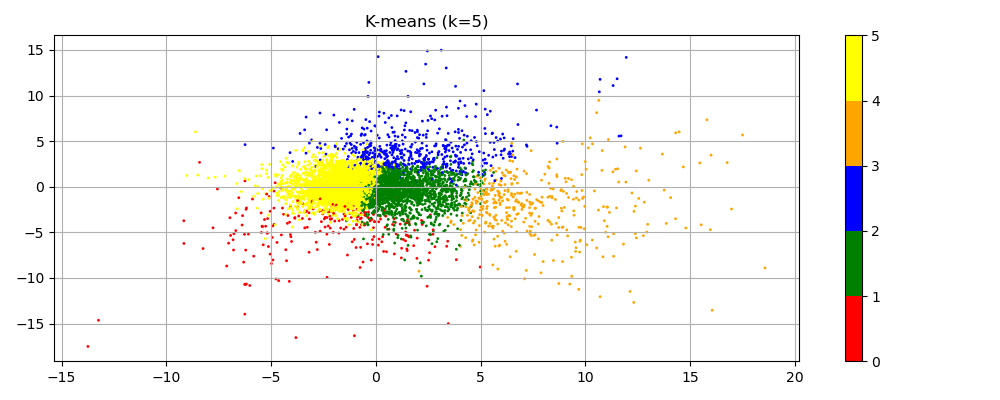
\includegraphics[width=1.0\textwidth]{kmeans_5}
		\caption{K-Means k=5}
		\label{fig:2.11}
	\end{minipage}%
	\begin{minipage}{.5\textwidth}
		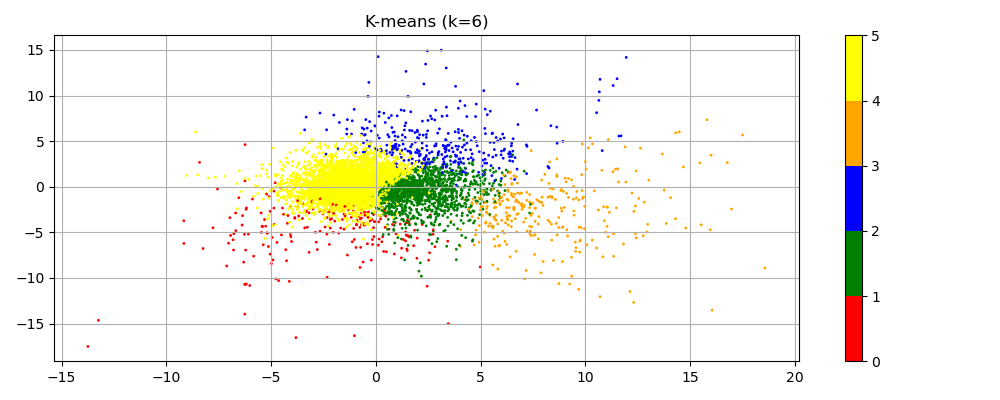
\includegraphics[width=1.0\textwidth]{kmeans_6}
		\caption{K-Means k=6}
		\label{fig:2.12}
	\end{minipage}
\end{figure}

K-Means also produces clusters. We can see the Voronoi graph as it divides the PCA 2-space neatly in K=3 and K=4. This tells me the clusters aren't seperable in 2-space - the values are filling the address space.

This is most similar to the Correlation Hierarchical cluster. If items are correlated, their vectors are in the same direction (but different magnitude). Since the n-space appears to be fully populated around a central point, this would closely match the Voronoi graph of K-means. It would fail when there are multiple clusters in a single direction at different magnitudes.

\section{Regression}

All the code is present in \(part3.R\). I didn't use the \(grid\) or \(thresh\) values, my search parameters produced better results. I used:

\begin{align}
	thresh &= 1e-12 \\
	grid &= 10^{seq(3,-2,length=100)}
\end{align}

\subsection{Random Seed}

The random seed was \(221\), which is set at the top of \(part3.R\) "\# Random Seed". \(part3.R\) is executeable via the makefile - \(make\ part3\), and creates the images and part3.txt with the output.

\subsection{Training/Test Set Split}

The \(model.matrix\) expression in the assignment wasn't used. It exhibits poor default behavior with nominal features and does not properly honour the train/test split.

For example, it assumes that there will only ever be two genders, and that NOT Female EQUALS Male. This is incorrect. It doesn't apply when there is a train/test split, it applies even less when there is a train/production split. For example, there are 3 genders on NZ Passports. The other nominal columns are treated the same way.

I used the \(recipes\) library instead. I pre-split the data into test/train datasets, created the transformation from the train dataset and applied it to the test dataset. This keeps the test data from applying a bias through the transformation to the model construction via value presence affecting column creation.

\subsection{How many predictors are there}

With a correct 1-hot transformation of nominal data \(p=120\). This could be improved with better handling of Yes/No columns, converting them to boolean first, avoiding one-hotting.

\subsection{Ridge Regression}

\begin{figure}[H]
	\includegraphics[width=0.25\textwidth]{ridge_model_lambda}
	\caption{Ridge Model Lambda}
	\label{fig:3.1}
\end{figure}

This is visible in part3.R under "\# Ridge Regression". The search algorithm found the minimal lamdba at \(0.367838\). 

\subsection{Lasso Regression}

\begin{figure}[H]
	\includegraphics[width=0.25\textwidth]{lasso_model_lambda}
	\caption{Lasso Model Lambda}
	\label{fig:3.2}
\end{figure}

This is visible in part3.R under "\# Lasso Regression". The search algorithm found the minimal lamdba at \(2.104904\). It selected 94 features, with 26 set to 0.

\subsection{Model Comparison}

Inspecting the model coefficients at the best lambda, the strongest predictors (highest coefficients) were:

\begin{table}[H]
	\centering
	\begin{tabular}{ | c | c | c | }
		\hline
		\textbf{Algorithm} & \textbf{Factor} & \textbf{oefficient} \\
		\hline
		Linear & Ethnicity\_Asian & 0.2905512 \\
		\hline
		Linear & Education & 0.5590759 \\
		\hline
		Linear & Gender\_X.Male & 12.5854597 \\
		\hline
		Linear & Cards & 21.9703714 \\
		\hline		
		Ridge & Student\_Yes & 7.615205e+01 \\
		\hline
		Ridge & Student\_Yes\_x\_Married\_Yes & 8.647941e+01  \\
		\hline
		Ridge & Gender\_Female\_x\_Student\_Yes & 9.282591e+01 \\
		\hline
		Ridge & Student\_Yes\_x\_Ethnicity\_Asian & 1.565377e+02 \\
		\hline
		Lasso & Married\_No\_x\_Ethnicity\_Caucasian & 8.439845e+00 \\
		\hline
		Lasso & Student\_Yes\_x\_Married\_No & 8.704450e+00 \\
		\hline
		Lasso & Cards\_x\_Student\_Yes & 1.276542e+01 \\
		\hline
		Lasso & Gender\_X.Male\_x\_Ethnicity\_Asian & 1.851114e+01 \\		
		\hline
	\end{tabular}
	\caption{Regression Error Comparison}
\end{table}

Linear regression picked a set of coefficients which don't particularly overlap with those selected by Ridge and Lasso. In Ridge and Lasso algorithms, Student\_Yes and Ethnicity\_Asian were strong predictors of balance. Additionally, the top predictors were pairs of values.

\subsection{Test Error Comparison}

\begin{table}[H]
	\centering
	\begin{tabular}{ | c | c | c | c | }
		\hline
		\textbf{Algorithm} & \textbf{MSE} & \textbf{RMSE} & \textbf{RSS} \\
		\hline
		Linear & 412,998.8131 & 642.6498 & 82,599,762.6255 \\
		\hline
		Ridge & 7,227.0139 & 85.0118 & 1,445,402.7827 \\
		\hline
		Lasso & 5,182.4367 & 71.9891 & 1,036,487.3454 \\
		\hline
	\end{tabular}
	\caption{Regression Error Comparison}
\end{table}

Lasso had the test error rates, with Linear regression significantly worse. Lasso had an approximately 30\% improvement in error magnitude.

\subsection{Test Predictions}

\begin{figure}[H]
	\includegraphics[width=0.4\textwidth]{all_on_one}
	\caption{Prediction Comparisons}
	\label{fig:3.3}
\end{figure}

If the predictions were correct, they should closely match the green X=Y line. Linear Regression is spreading data all around. Both Ridge and Lasso are attempting to predict the data, but are failing to predict values where the balance is zero, predicting negative values. We can also see that Lasso is tighter to the Y=X line than Ridge, reflecting the error results.

\section{Appendix - Figures}


\begin{figure}[H]
	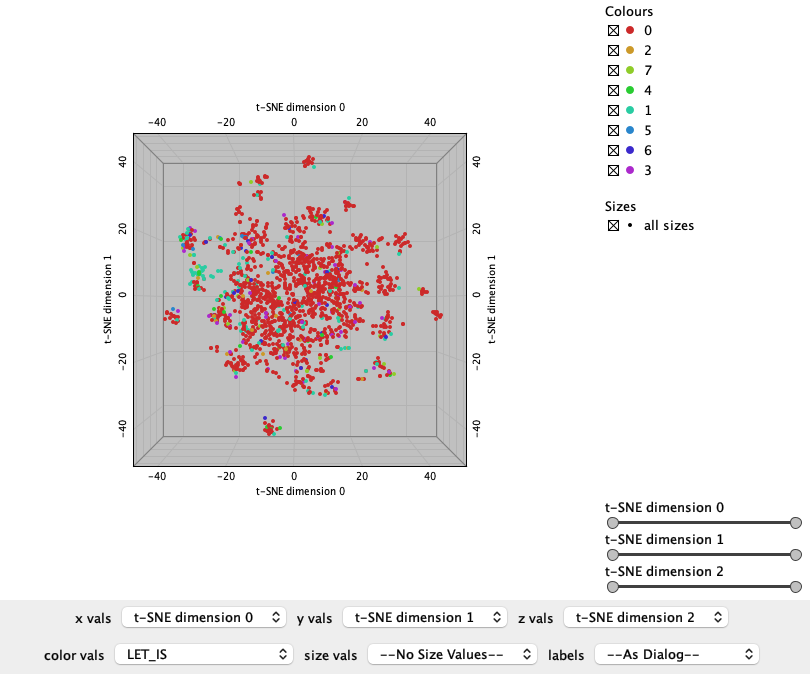
\includegraphics[width=1.0\textwidth]{t-sne-iter100k}
	\caption{t-SNE 100k iterations}
	\label{fig:1.5}
\end{figure}

\begin{figure}[H]
	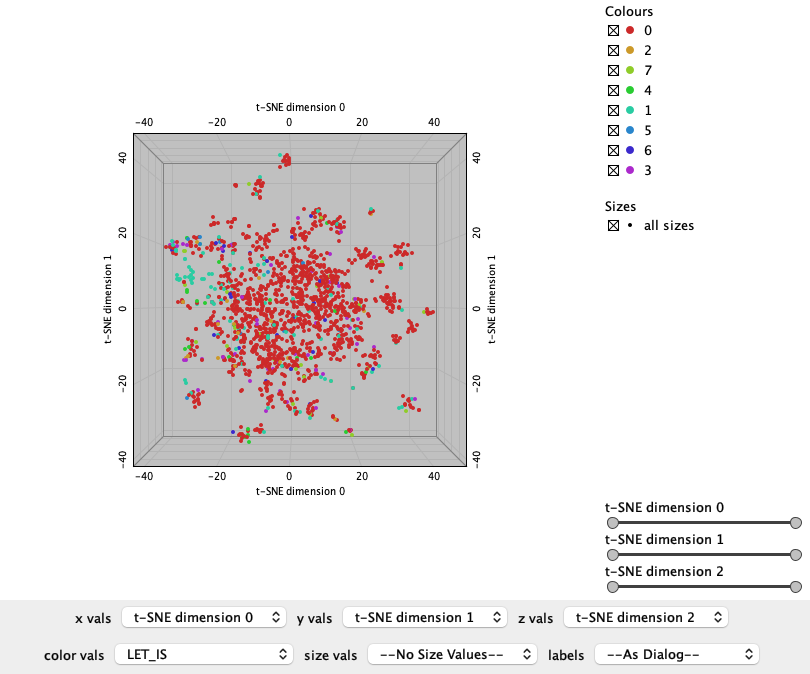
\includegraphics[width=1.0\textwidth]{t-sne-iter50k}
	\caption{t-SNE 50k iterations}
	\label{fig:1.6}
\end{figure}

\begin{figure}[H]
	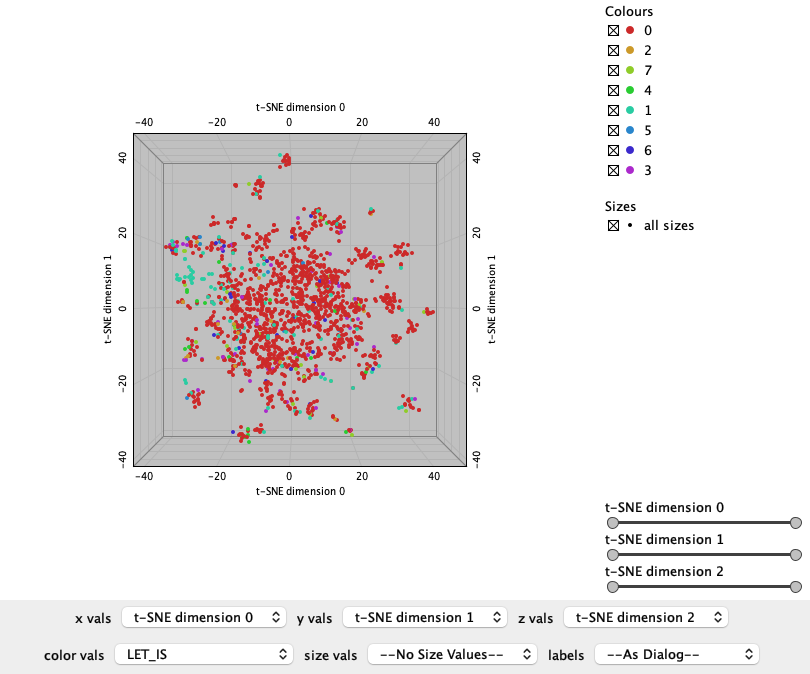
\includegraphics[width=1.0\textwidth]{t-sne-iter10k}
	\caption{t-SNE 10k iterations}
	\label{fig:1.7}
\end{figure}

\begin{figure}[H]
	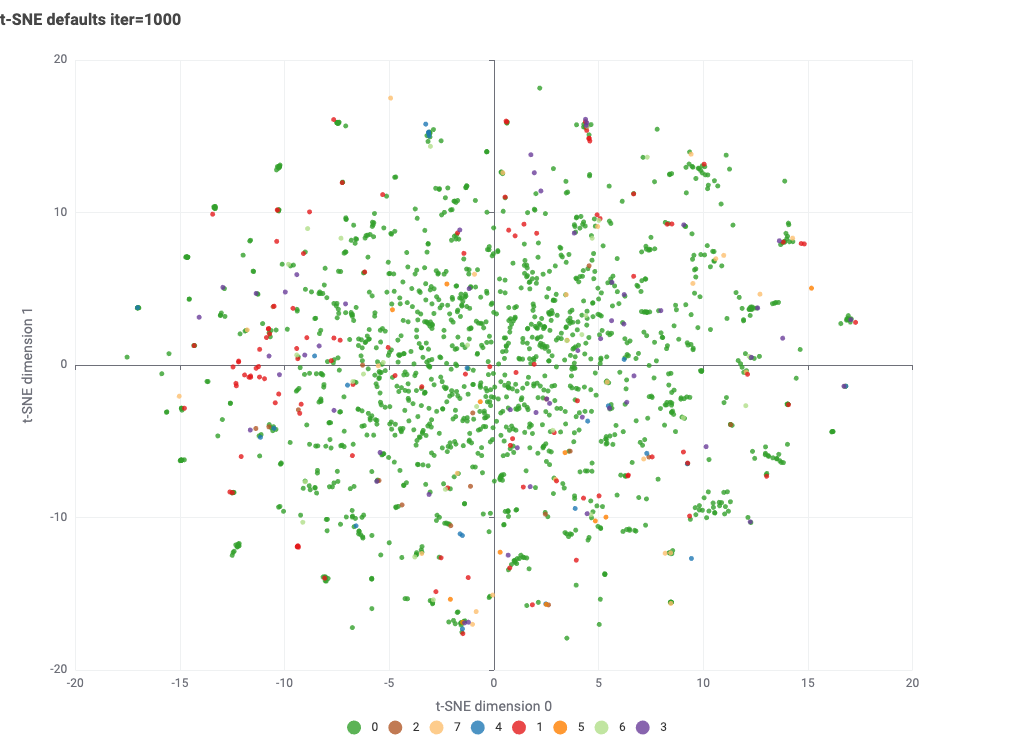
\includegraphics[width=1.0\textwidth]{t-sne-iter1k}
	\caption{t-SNE 1k iterations}
	\label{fig:1.8}
\end{figure}

\begin{figure}[H]
	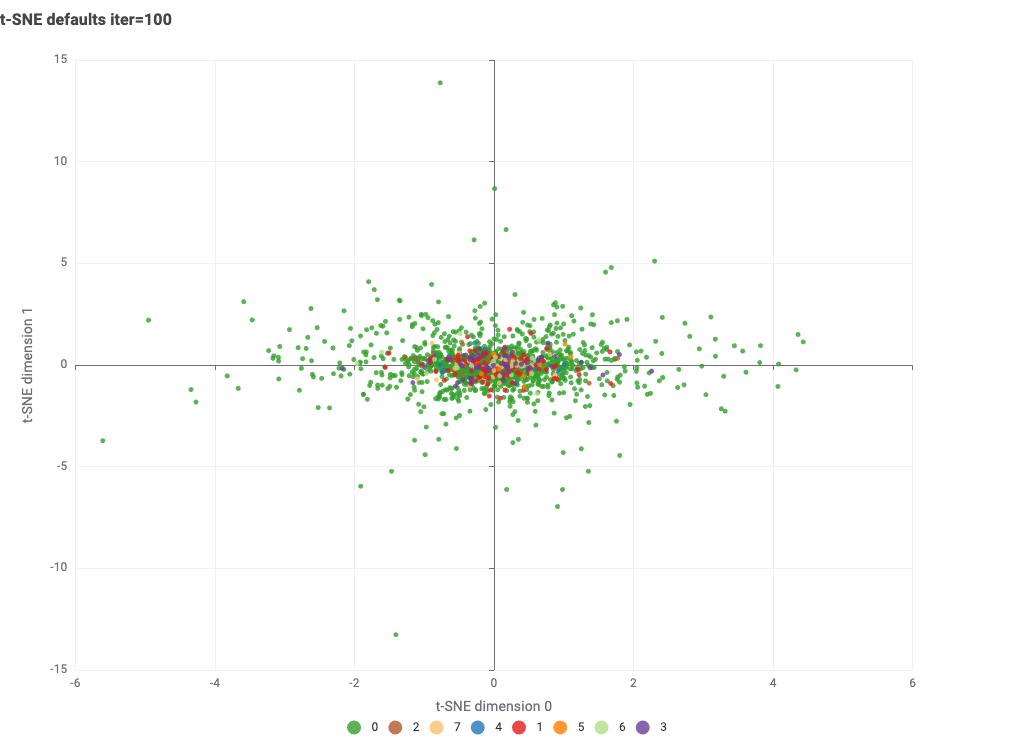
\includegraphics[width=1.0\textwidth]{t-sne-iter100}
	\caption{t-SNE 100 iterations}
	\label{fig:1.9}
\end{figure}

\begin{figure}[H]
	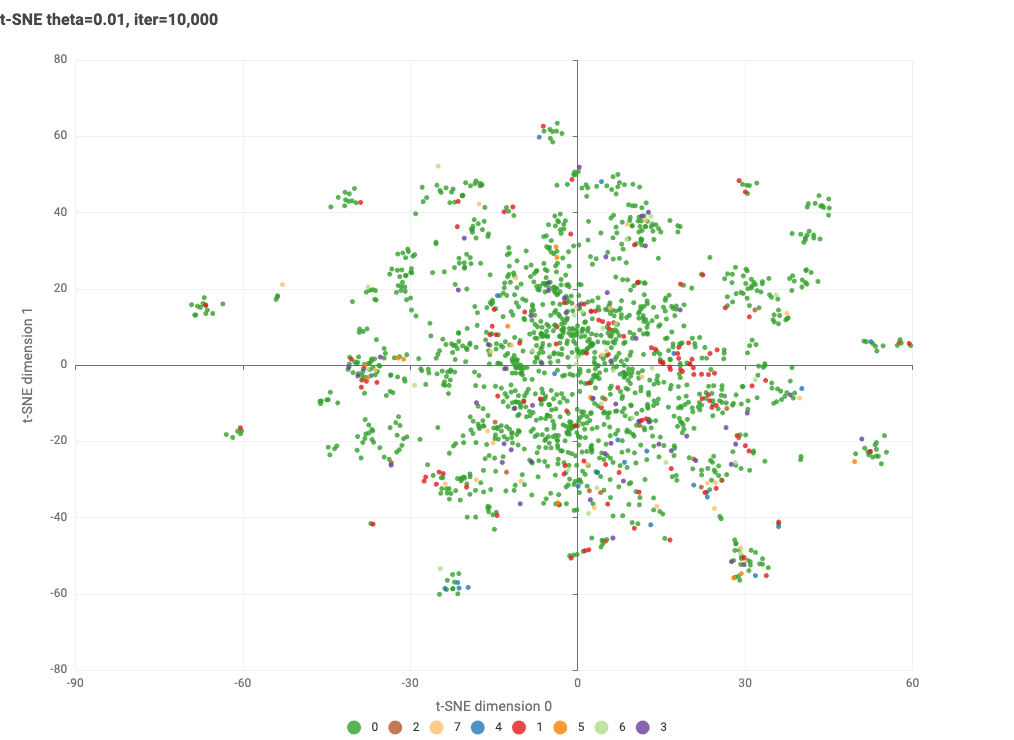
\includegraphics[width=1.0\textwidth]{t-sne-iter10k-theta0-01}
	\caption{t-SNE 10k iterations, theta 0.01}
	\label{fig:1.10}
\end{figure}

\begin{figure}[H]
	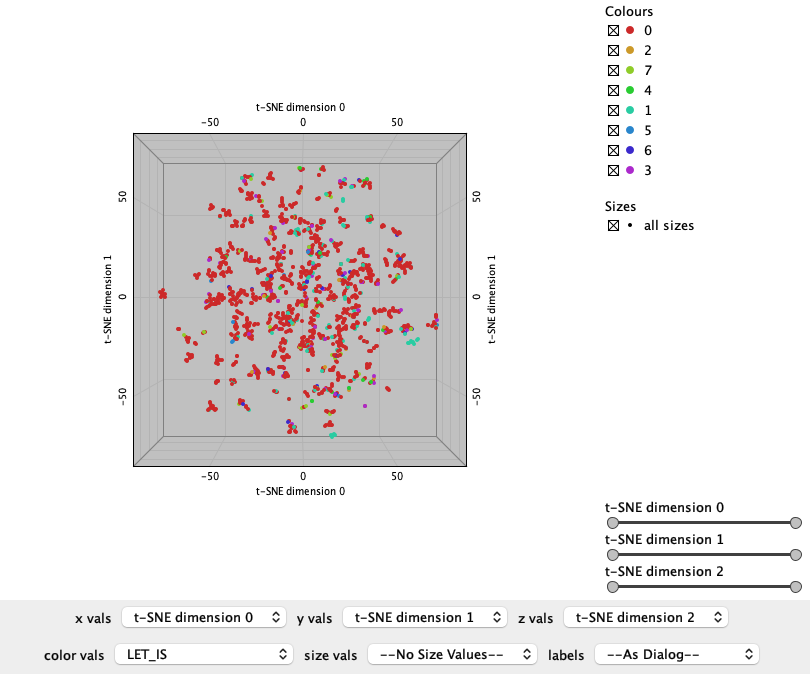
\includegraphics[width=1.0\textwidth]{t-sne-iter10k-theta0-01-perplexity2}
	\caption{t-SNE 10k iterations, theta 0.01, perplexity 2}
	\label{fig:1.11}
\end{figure}

\begin{figure}[H]
	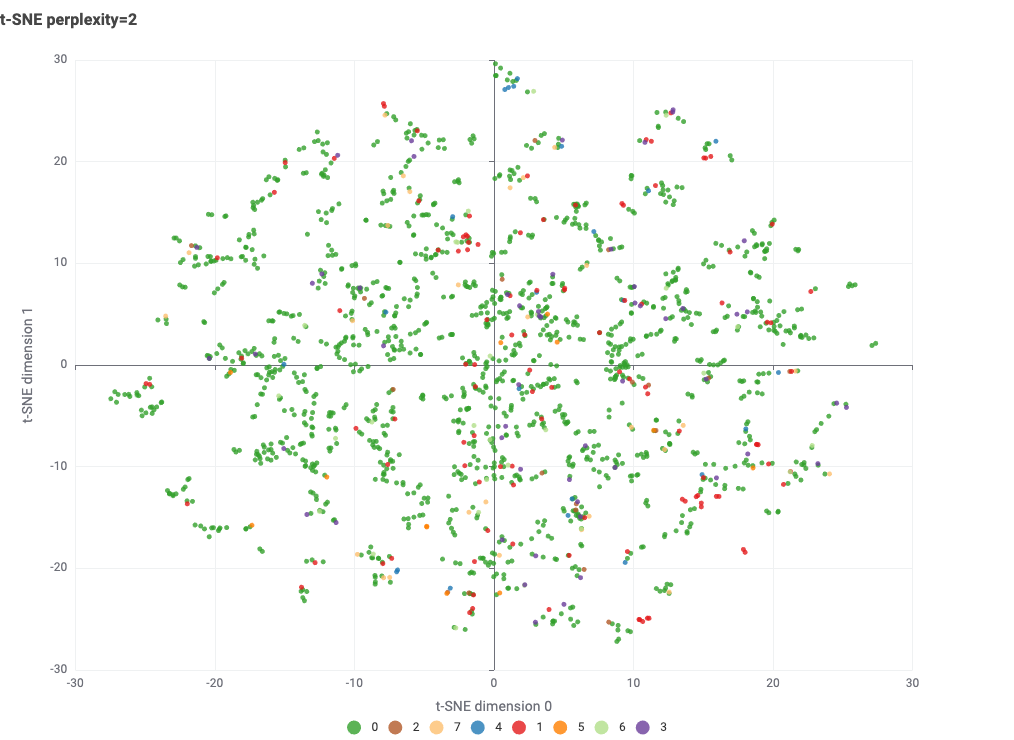
\includegraphics[width=1.0\textwidth]{t-sne-perplexity2}
	\caption{t-SNE perplexity 2}
	\label{fig:1.12}
\end{figure}

\begin{figure}[H]
	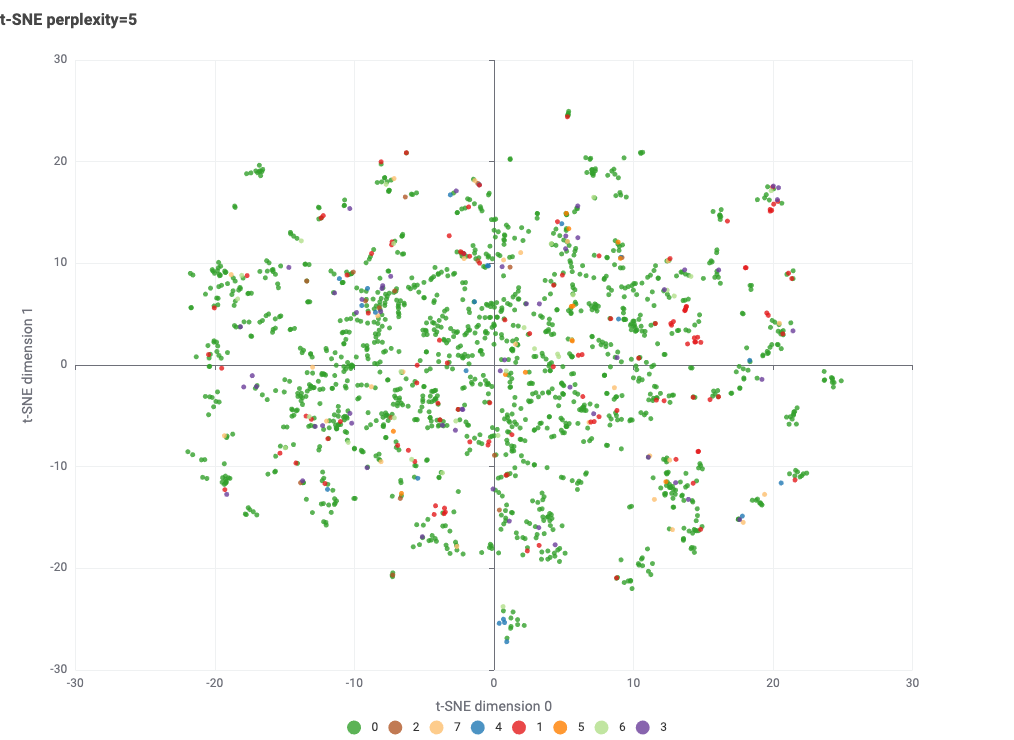
\includegraphics[width=1.0\textwidth]{t-sne-perplexity5}
	\caption{t-SNE perplexity 5}
	\label{fig:1.13}
\end{figure}

\begin{figure}[H]
	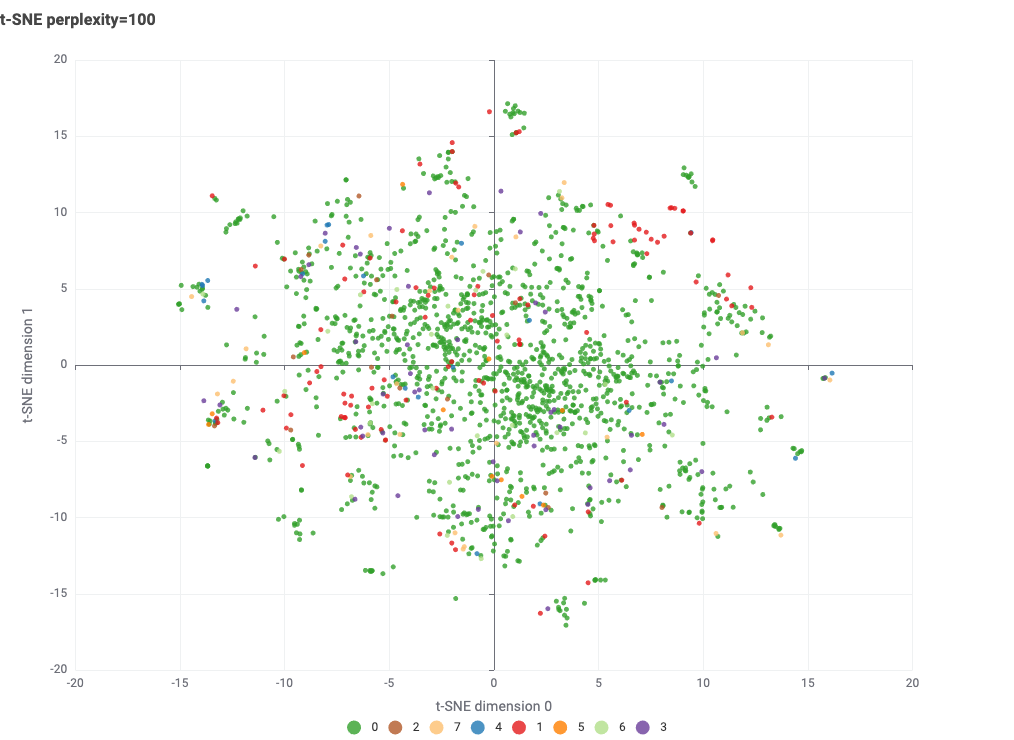
\includegraphics[width=1.0\textwidth]{t-sne-perplexity100}
	\caption{t-SNE perplexity 100}
	\label{fig:1.14}
\end{figure}

\subsection{Appendix - Code}

\begin{figure}[H]
	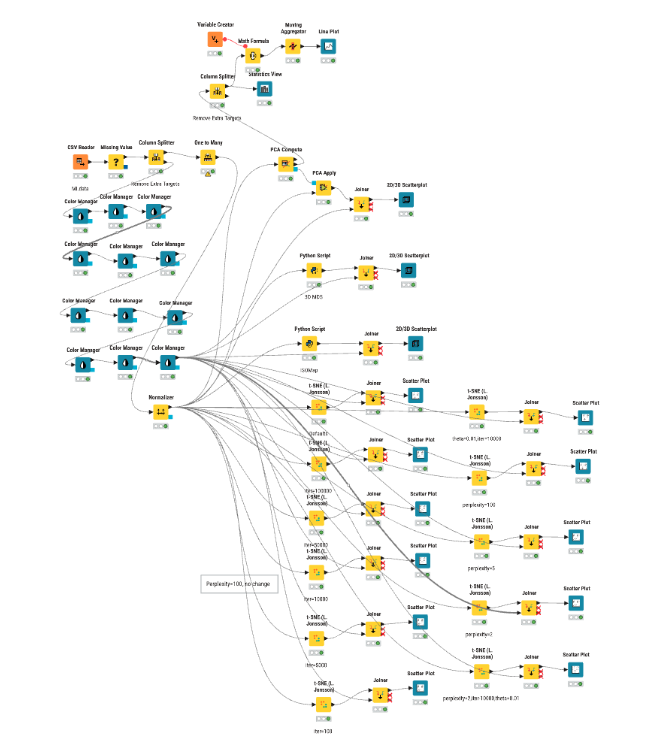
\includegraphics[width=1.0\textwidth]{knime-flow}
	\caption{Question 1, KNime workflow}
	\label{fig:1.15}
\end{figure}

Python code used to generate MDS and variances.

\begin{lstlisting}[language=Python]
	import knime.scripting.io as knio
	import pandas as pd
	import numpy as np
	from sklearn.manifold import MDS
		
	input_table_1 = knio.input_tables[0].to_pandas()

	n_components = 3
	dissimilarity = 'euclidean'
	
	mds_manifold = MDS(n_components=n_components, dissimilarity=dissimilarity)
	transformed = mds_manifold.fit_transform(input_table_1)
	output_dataframe = pd.DataFrame(transformed, index=input_table_1.index)


	incoming_variance=np.var(input_table_1, axis=0)
	total_incoming_variance=incoming_variance.sum()
	knio.flow_variables['total_incoming_variance'] = f"{total_incoming_variance}"

	outgoing_variance=np.var(output_dataframe)
	total_outgoing_variance = outgoing_variance.sum()
	knio.flow_variables['total_outgoing_variance'] = f"{total_outgoing_variance}"

	knio.output_tables[0] = knio.Table.from_pandas(output_dataframe)
\end{lstlisting}
\end{document}